\chapter{Sensores de Temperatura}

La medida de la temperatura es una de las más comunes y de las más importantes que se efectúan en los procesos industriales. Casi todos los fenómenos físicos están afectados por ella. 

Existen diversos fenómenos que son influidos por la temperatura y que son utilizados para medirla:
\begin{itemize}
    \item Variaciones en volumen o en estado de los cuerpos (sólidos, líquidos o gases).
    \item Variación de resistencia de un conductor (sondas de resistencia).
    \item Variación de resistencia de un semiconductor (termistores).
    \item La fuerza electromotriz creada en la unión de dos metales distintos (termopares).
    \item Intensidad de la radiación total emitida por el cuerpo (pirómetros de radiación).
    \item Otros fenómenos utilizados en laboratorio (velocidad del sonido en un gas, frecuencia de resonancia de un cristal, etc.)
\end{itemize}
De este modo, se emplean los siguientes instrumentos: termómetros de vidrio, termómetros bimetálicos, elementos primarios de bulbo y capilar rellenos de líquido, gas o vapor, termómetros de resistencia, termopares, pirómetros de radiación, termómetros ultrasónicos y termómetros de cristal de cuarzo.

\section{Termómetro de vidrio}
El termómetro de vidrio consta de un depósito de vidrio que contiene, por ejemplo, mercurio (-35ºC hasta 280ºC), pentano (-200ºC hasta 20ºC) o alcohol (-110ºC hasta 50ºC) y que al calentarse, se expande y sube en el tubo capilar.

\begin{figure} [H]
    \centering
    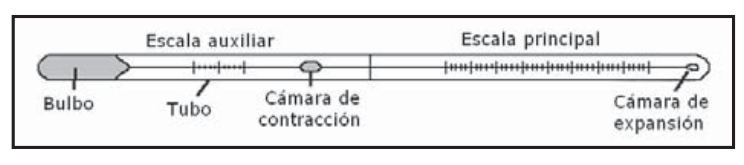
\includegraphics[width=0.5\linewidth]{Imagenes/Termometro de vidrio.png}
    \caption{Termómetro de vidrio}
\end{figure}

\section{Termómetro bimetálico}
Los termómetros bimetálicos se fundamentan en el distinto coeficiente de dilatación de dos metales diferentes laminados conjuntamente, que se deforma cuando se produce un cambio de temperatura.

\section{Termómetros de bulbo y capilar}
Los termómetros tipo bulbo y capilar consisten, esencialmente, en un bulbo conectado por un capilar a una espiral. Cuando la temperatura del bulbo cambia, el gas o el líquido en el bulbo se expande y la espiral tiende a desenrollarse, moviendo la aguja sobre la escala para indicar la elevación de la temperatura en el bulbo.
Hay cuatro clases de este tipo de termómetros:
\begin{itemize}
    \item Clase I. Termómetros actuados por líquido.
    \item Clase II. Termómetros actuados por vapor.
    \item Clase III. Termómetros actuados por gas.
    \item Clase IV. Termómetros actuados por mercurio.
\end{itemize}

\section{Termómetros de resistencia}
La medida de temperatura utilizando sondas de resistencia depende de la variación de resistencia en función de la temperatura, que es propia del elemento de detección. 

El elemento consiste, usualmente, en un arrollamiento de hilo muy fino del conductor adecuado bobinado entre capas de material aislante y protegido con un revestimiento de vidrio o de cerámica.

El material que forma el conductor se caracteriza por el llamado "coeficiente de temperatura de resistencia" que expresa, a una temperatura especificada, la variación de la resistencia en ohmios del conductor por cada grado que cambia su temperatura.

La relación entre estos factores puede verse en la siguiente expresión lineal:
\begin{equation}
    R_t = R_0 (1 + \alpha t)
\end{equation}

\begin{figure}[H]
    \centering
    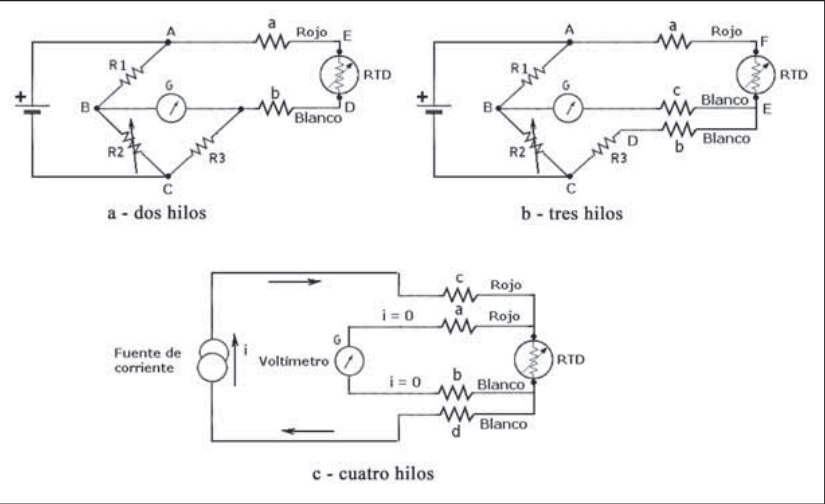
\includegraphics[width=0.5\linewidth]{Imagenes/Termometros de resistencia.png}
    \caption{Tipos de circuitos de puente de Wheatstone a sonda de resistencia.}
\end{figure}

La medición automática clásica de la resistencia y, por lo tanto, de la temperatura se lleva a cabo mediante instrumentos auto equilibrados que utilizan un circuito de puente de Wheatstone o bien un puente de capacidades.

En ambos casos, un motor de equilibrio es excitado siempre que el puente esté equilibrado, de tal modo que el instrumento está marcando continuamente la temperatura del proceso.
La adición de un convertidor o transductor permite obtener una tensión proporcional a la resistencia, que puede amplificarse. Añadiendo transmisión de datos vía bus se obtiene un "transmisor inteligente" con la posibilidad del cambio automático del sensor o del campo de medida, la obtención por hardware o por software de diferentes características, etc.
\section{Termistores}
Los termistores son semiconductores electrónicos con un coeficiente de temperatura de resistencia negativo de valor elevado, por lo que presentan unas variaciones rápidas, y extremadamente grandes, para los cambios, relativamente pequeños, en la temperatura.

Los termistores también se denominan NTC (\textit{Negative Temperature Coeficient}) existiendo casos especiales de coeficiente positivo cuando su resistencia aumenta con la temperatura (PTC - \textit{Positive Temperature Coeficient})

La relación entre la resistencia del termistor y la temperatura viene dada por la expresión:
\begin{equation}
    R_t = R_0 e^{\beta \left( \frac{1}{T_t} - \frac{1}{T_0} \right)}
\end{equation}

Los termistores se conectan a puentes de Wheatstone convencionales o a circuitos que convierten su resistencia a una tensión de salida proporcional. La distancia entre el termistor y el instrumento de medida puede ser considerable siempre que el elemento posea una alta resistencia comparada con la de los cables de unión. La corriente que circula por el termistor, a través del circuito de medida, debe ser baja para garantizar que la variación de resistencia del elemento sea debida exclusivamente a los cambios de temperatura en el proceso.

\section{Termopares}

Cuando el termopar está instalado a una distancia larga del instrumento, no se conecta directamente al mismo, sino por medio de un cable de extensión o compensación. (Figura \ref{fig:termopares}). Los cables de extensión son conductores con propiedades eléctricas similares a las del termopar a las temperaturas límites que pueden encontrarse en el proceso y son más económicos. El uso del cable de extensión es claro en el caso de termopares tipo R o S, debido al elevado precio del platino que encarecería el coste del hilo desde el campo hasta el panel.

\begin{figure}[H]
    \centering
    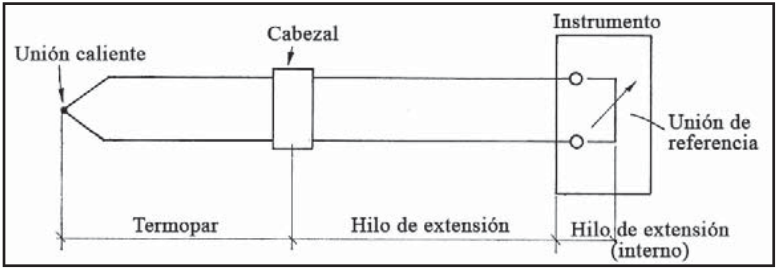
\includegraphics[width=0.5\linewidth]{Imagenes/Termopares.png}
    \caption{Diagrama de un sistema pirométrico}
    \label{fig:termopares}
\end{figure}

En los instrumentos clásicos galvanométricos o potenciométricos, la compensación se realiza mediante una resistencia (resistencia de compensación de la unión fría), que absorbe una tensión equivalente a la f.e.m. que tendría el termopar con la unión caliente a la temperatura de la caja del instrumento y la unión fría a 0ºC
En los instrumentos digitales se utilizan módulos de acondicionamiento que compensan, electrónicamente, el cambio de temperatura de la unión fría y que, además, linealizan, con relación a la temperatura, los mV generados por el termopar.
\begin{figure}
    \centering
    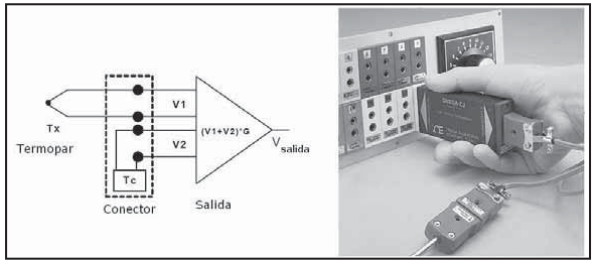
\includegraphics[width=0.5\linewidth]{Imagenes/Termopar.png}
    \caption{Módulo de compensación de la unión fría del termopar.}
    \label{fig:enter-label}
\end{figure}

\section{Pirómetros de radiación}
Los pirómetros de radiación se fundan en la ley de Stefan-Boltzmann, que dice que la intensidad de energía radiante emitida por la superficie de un cuerpo aumenta proporcionalmente a la cuarta potencia de la temperatura absoluta (Kelvin) del cuerpo, es decir:
\begin{equation}
    W = K \times T^4
\end{equation}

Los pirómetros de radiación miden, pues, la temperatura de un cuerpo a distancia en función de su radiación. Existen varios tipos, el pirómetro óptico que capta la radiación luminosa entre 0,4 a 0,7 micras, el pirómetro de infrarrojos de 0,7 a 20 micras, el detector fotoeléctrico que mide la radiación térmica, el pirómetro de dos colores o de relación entre radiaciones correspondientes a dos bandas estrechas y el pirómetro de radiación total, que mide toda la radiación emitida por el cuerpo.

\section{Pirómetros ópticos}
Los pirómetros ópticos automáticos son parecidos a los de la radiación infrarroja. Comparan la radiación emitida por el cuerpo con la emitida por una fuente de referencia controlada. Consisten, esencialmente, en un disco rotativo que expone el detector a la radiación del objeto y a la de referencia, alternativamente. La exactitud de los pirómetros ópticos es del $\pm$ 1 \% al $\pm$ 2\%.

\section{Sensores monolíticos}
% Pendiente de encontrar 